\chapter{SciPy による数値計算とフィット}
\label{chap:scipy}

SciPy\index{scipy@SciPy|textbf} は、データに式を当てはめる計算や、分布の推定などに使うライブラリである。この章では、まず 5 個の点に合う直線を求める。その後で分布、重み付け、補間、波形処理を学ぶ。求めた値を図へ重ね、データとのずれと適用条件を確かめられるようにする。

本章の例を試すには、第~\ref{chap:setup}~章で用意した仮想環境を使う。ターミナル（Windows では Ubuntu の端末）で次を入力し、本章用のフォルダーへ移動する。

\begin{lstlisting}[numbers=none, xleftmargin=2\zw]
$ source ~/analysis_practice/.venv/bin/activate
$ mkdir -p ~/analysis_practice/scipy
$ cd ~/analysis_practice/scipy
\end{lstlisting}

以降、ファイル名だけで指定した保存先や入力元は、このフォルダー内を指す。

\section{データに直線を当てはめる}

\subsection{データに合う直線を求める}

横軸を \code{x}、縦軸を \code{y} としてデータを描くと、点がおおむね直線に沿って並ぶ場合がある。そこで、直線を表す式 \code{y = a * x + b} を使い、点の並びに合う \code{a} と \code{b} を求める。

\code{a} は直線の傾き、\code{b} は \code{x = 0} のときの \code{y} の値である。このように、データに合わせて式の中の値を求めることを「フィット」という。ここでは、各点の \code{y} と直線の \code{y} の差を二乗し、その合計が小さくなるように \code{a} と \code{b} を求める。

式の中で調整する \code{a} と \code{b} をパラメータという。観測値から式による値を引いた差を残差という。求めた直線をデータと同じ図に描き、各点とのずれを確かめる。次の \code{curve\_fit()} の例で、この 2 つの値を計算する。

直線を使ってよいかは、データが得られた過程や図の形に基づいて判断する。推定値の解釈には、使った範囲、残差、推定値の不確かさの確認も必要である。重み付けや共分散による評価は、基本のフィットを試した後に説明する。

\subsection{\code{curve\_fit} によるパラメータ推定}

次の動作確認用のデータでは、傾きと切片を持つ直線を当てはめる。\code{linear\_model(x, a, b)} に \code{x} と候補の \code{a}、\code{b} を渡すと、直線上の \code{y} が返る。\code{curve\_fit()} はこの関数を繰り返し呼び、データとの差の二乗和が小さくなる \code{a} と \code{b} を探す。次を \code{fit\_line.py} へ保存し、端末で \code{python fit\_line.py} を実行する。

\noindent\begin{minipage}{\linewidth}
\begin{lstlisting}[language=Python]
import numpy as np
from scipy.optimize import curve_fit

def linear_model(x, a, b):
    return a * x + b

xdata = np.array([0.0, 1.0, 2.0, 3.0, 4.0])
ydata = np.array([1.1, 2.0, 3.2, 4.1, 5.1])

linear_params, linear_cov = curve_fit(linear_model, xdata, ydata)
linear_errors = np.sqrt(np.diag(linear_cov))

print(linear_params)
print(linear_errors)
\end{lstlisting}
\end{minipage}

最初の行が傾きと切片、次の行がそれぞれの標準誤差である。標準誤差は、仮定した誤差モデルの下で推定値がどの程度変わり得るかの目安であり、その計算は後で説明する。まず傾きが約 1.01、切片が約 1.08 になったことを確認する。

\begin{lstlisting}[numbers=none, xleftmargin=2\zw]
[1.01 1.08]
[0.02516611 0.06164414]
\end{lstlisting}

\code{linear\_params} は推定した傾きと切片である。\code{linear\_cov} は、それらの不確かさを 2 行 2 列にまとめた共分散行列である。左上と右下を対角成分と呼び、それぞれ傾きと切片の分散を表す。\code{np.diag(linear\_cov)} はこの 2 個を取り出し、\code{np.sqrt(...)} は平方根を求めるため、各パラメータの標準誤差が得られる。上の例では \code{linear\_params[0]} が傾き、\code{linear\_params[1]} が切片である。非対角成分はパラメータ間の共分散を表すため、相関を調べる場合は各パラメータの標準偏差で規格化する。\code{curve\_fit()} の出力は、仮定したモデル、残差の定義、\code{sigma} の指定に依存する。

上の直線モデル \(f(x; a, b) = ax + b\) なら、\code{curve\_fit()} は概ね
\[
S(a, b) = \sum_i \left[y_i - (a x_i + b)\right]^2
\]
を小さくする \(a\) と \(b\) を探していると考えればよい。より一般には、モデル \(f(x; \mathbf{p})\) に対して
\[
S(\mathbf{p}) = \sum_i \left[y_i - f(x_i; \mathbf{p})\right]^2
\]
という残差二乗和を最小化している。

直線が点の並びに合っているかを確かめるため、\code{fit\_line.py} の末尾へ次を追記して再実行する。作業フォルダーにできた \code{linear\_fit.pdf} を開き、測定点と直線の位置を見比べる。

\begin{lstlisting}[language=Python]
import matplotlib.pyplot as plt

fig, ax = plt.subplots()
ax.scatter(xdata, ydata, label="data")
ax.plot(xdata, linear_model(xdata, linear_params[0], linear_params[1]), label="fit")
ax.set_xlabel("x")
ax.set_ylabel("y")
ax.legend()
fig.savefig("linear_fit.pdf")
\end{lstlisting}

数値が得られたことだけでは、直線を使ってよいとは判断できない。残差の並びや測定条件も確認する方法を、後の節で学ぶ。

\section{分布と要約統計}

\subsection{NumPy 配列を入力とする専門計算機能}

SciPy の多くの関数は NumPy 配列を入力とし、NumPy 配列またはスカラーを返す。したがって、入力の \code{shape} と \code{dtype}、返り値の意味を NumPy の配列操作と対応付ける。SciPy 内で目的別に分けた機能のまとまりをサブパッケージといい、次のように選ぶ。

\begin{itemize}
\item \code{scipy.stats}\index{scipy@SciPy!stats@\code{scipy.stats}|textbf}: 分布、検定、要約統計
\item \code{scipy.optimize}: 最適化、非線形最小二乗、\code{curve\_fit}\index{scipy@SciPy!curve\_fit@\code{curve\_fit}|textbf}
\item \code{scipy.interpolate}\index{scipy@SciPy!interpolate@\code{scipy.interpolate}|textbf}: 補間
\item \code{scipy.signal}\index{scipy@SciPy!signal@\code{scipy.signal}|textbf}: フィルタ、ピーク検出、相関、スペクトル処理
\item \code{scipy.integrate}\index{scipy@SciPy!integrate@\code{scipy.integrate}|textbf}: 数値積分
\item \code{scipy.constants}\index{scipy@SciPy!constants@\code{scipy.constants}|textbf}: 物理定数
\end{itemize}

要素ごとの演算や基本的な集計には NumPy を用い、確率分布、最適化、補間、信号処理などの専用アルゴリズムが必要な場合に、対応する SciPy のサブパッケージを選ぶ。

\subsection{正規分布と指数分布}

多数の独立な微小変動の和は、条件を満たせば正規分布で近似できる。事象が互いに独立に一定の発生率で起こる Poisson（ポアソン）過程では、事象間の待ち時間が指数分布に従う。対象データがこれらの仮定を満たすかは、生成過程、残差、代替モデルとの比較によって検証する。

たとえば、平均 \(\mu\)、標準偏差 \(\sigma\) のガウシアンは
\[
p(x) = \frac{1}{\sqrt{2\pi}\sigma}
\exp\!\left[-\frac{(x-\mu)^2}{2\sigma^2}\right]
\]
で書ける。また、時定数 \(\tau\) の指数分布は
\[
p(t) = \frac{1}{\tau} \exp\!\left(-\frac{t}{\tau}\right)
\qquad (t \ge 0)
\]
である。SciPy の分布オブジェクトは、確率密度、累積分布、分位点、乱数生成を共通のインタフェースで提供する。

\subsection{\code{scipy.stats} による要約統計と分布}

配列の要素数、中心、広がり、形状を数値で確認する方法を示す。

\begin{lstlisting}[language=Python]
import numpy as np
from scipy import stats

values = np.array([1.2, 0.9, 1.5, 1.1, 0.8])

summary = stats.describe(values)
print(summary.nobs)
print(f"{summary.mean:.3f}")
print(f"{summary.variance:.3f}")
\end{lstlisting}

この例では、要素数、平均、分散が順に表示される。

\begin{lstlisting}[numbers=none, xleftmargin=2\zw]
5
1.100
0.075
\end{lstlisting}

\code{stats.describe()} は、要素数、平均、分散、最小値、最大値、歪度、尖度を名前付きタプルとして返す。分散の既定は \code{ddof=1} であり、NumPy の \code{var()} の既定とは異なる。各統計量の定義と単位を確認してから利用する。

SciPy の分布オブジェクトは、確率密度関数や累積分布関数を同じ API で扱える。

\begin{lstlisting}[language=Python]
x = np.linspace(-3.0, 3.0, 7)
pdf = stats.norm.pdf(x, loc=0.0, scale=1.0)
cdf = stats.norm.cdf(x, loc=0.0, scale=1.0)

print(pdf)
print(cdf)
\end{lstlisting}

\code{pdf} と \code{cdf} を同じ点列で評価すると、次のような値が得られる。

\begin{lstlisting}[numbers=none, xleftmargin=2\zw]
[0.00443185 0.05399097 0.24197072 0.39894228 0.24197072 0.05399097
 0.00443185]
[0.0013499  0.02275013 0.15865525 0.5        0.84134475 0.97724987
 0.9986501 ]
\end{lstlisting}

\code{pdf} は確率密度関数、\code{cdf} は累積分布関数、\code{rvs} は乱数生成、\code{ppf} は累積確率から分位点を求める逆関数に対応する。正規分布では \code{loc} は平均、\code{scale} は標準偏差であるが、これらの引数の意味は分布ごとに確認する。

ここで \code{pdf} は確率密度 \(p(x)\)、\code{cdf} はその積分
\[
F(x) = \int_{-\infty}^{x} p(t)\,dt
\]
に対応する。したがって、\code{stats.norm.cdf(x)} は「\(x\) 以下に入る確率」を返している。

\section{モデル選択・重み付け・残差評価}

モデル推定では、次の項目を順に記録する。

\begin{enumerate}
\item 作図に基づく候補関数の検討
\item フィット範囲の決定
\item 必要に応じた妥当な初期値の設定
\item データとフィット曲線の重ね描き
\item 推定値と残差の確認
\end{enumerate}

モデルの定義とデータの確認を省いて \code{curve\_fit()} を実行しても、推定値の妥当性を判断できない。フィットは、モデルという仮説をデータと残差によって検証する手続きである。

\subsection{初期値、制約、残差}

モデルによっては、初期値や制約を与えないと不安定になる。

\begin{lstlisting}[language=Python]
def exp_model(x, a, tau, c):
    return a * np.exp(-x / tau) + c

x_decay = np.linspace(0.0, 8.0, 40)
rng = np.random.default_rng(31)
y_decay = 4.0 * np.exp(-x_decay / 2.5) + 0.3
y_decay += rng.normal(loc=0.0, scale=0.05, size=x_decay.size)

exp_params, exp_cov = curve_fit(
    exp_model,
    x_decay,
    y_decay,
    p0=[5.0, 2.0, 0.0],
    bounds=([0.0, 0.0, -np.inf], [np.inf, np.inf, np.inf]),
)
\end{lstlisting}

\code{p0}\index{p0@\code{p0}|textbf} は初期値、\code{bounds}\index{bounds@\code{bounds}|textbf} はパラメータ範囲である。どちらも収束を保証するものではないが、物理的にあり得ない範囲を除外する際に有効である。モデルによっては、初期値によって収束先が変わる。また、物理的に非負であるパラメータには、0 を下限とする制約を指定できる。

フィット結果の図には、関数形、推定パラメータ、データ系列を識別できる情報を記載する。凡例を用いる場合は、データや曲線を隠さない位置を選び、複数の図で同じ書式を用いる。

\begin{lstlisting}[language=Python]
import numpy as np
import matplotlib.pyplot as plt
from scipy import stats

rng = np.random.default_rng(37)
values = rng.normal(loc=3.0, scale=0.8, size=3000)
mean, sigma = stats.norm.fit(values)
x = np.linspace(values.min(), values.max(), 300)

fig, ax = plt.subplots()
ax.hist(values, bins=40, density=True, alpha=0.7, label="sample")
ax.plot(
    x,
    stats.norm.pdf(x, loc=mean, scale=sigma),
    linewidth=2.0,
    label=(
        "fit: "
        r"$f(x)=\frac{1}{\sqrt{2\pi}\sigma}"
        r"\exp\!\left[-\frac{(x-\mu)^2}{2\sigma^2}\right]$"
        "\n"
        + fr"$\mu={mean:.2f},\ \sigma={sigma:.2f}$"
    ),
)
ax.legend(loc="upper right")
\end{lstlisting}

図~\ref{fig:distribution-examples} では、フィットした分布名と推定パラメータを凡例へ記載している。左パネルは上の正規乱数と同じ入力を用い、右パネルは同じ乱数生成器で続けて生成した時定数 2.5 s、3000 個の指数乱数を用いる。本文には推定方法と解釈、キャプションには図の対象と条件、凡例には系列の識別情報を置く。

\begin{lstlisting}[language=Python]
model_y = linear_model(xdata, *linear_params)
residual = ydata - model_y
print(residual)
\end{lstlisting}

最適化が終了して推定値を返したことは、モデルの妥当性を保証しない。残差を横軸に対して表示し、符号や大きさに系統的な構造が残っていないか、特定の範囲だけ偏差が大きくないかを確認する。

外れ値やモデルの適用範囲外にある領域を含めると、推定値が変化する場合がある。フィット範囲と除外条件を推定値とともに記録する。

\begin{lstlisting}[language=Python]
mask = (xdata >= 0.0) & (xdata <= 3.0)
range_params, range_cov = curve_fit(
    linear_model,
    xdata[mask],
    ydata[mask],
)
\end{lstlisting}

フィット範囲は、モデルを適用する領域を定義する解析条件である。範囲をデータ確認後に変更した場合は、その判断基準と変更前後の結果も報告する。

\subsection{\code{sigma} を使った重み付きフィット}

物理の実データでは、各データ点の不確かさが等しいとは限らない。点ごとの標準偏差が既知であり、その大きさが異なる場合は、\code{sigma}\index{sigma@\code{sigma}|textbf} を使って残差を標準偏差で割る。このように比較の基準となる大きさで割る操作を、ここでは規格化と呼ぶ。同じ 1 のずれでも、標準偏差が 0.5 なら規格化した残差は 2、標準偏差が 2 なら 0.5 となる。\code{sigma} を与えないフィットはすべての点を等しい重みで扱うため、不確かさが点ごとに異なるデータでは目的と一致しない場合がある。

\begin{lstlisting}[language=Python]
y_err = np.array([0.2, 0.2, 1.5, 0.2, 0.2])

weighted_params, weighted_cov = curve_fit(
    linear_model,
    xdata,
    ydata,
    sigma=y_err,
    absolute_sigma=True,
)
\end{lstlisting}

この定義では、\code{sigma} が大きい点ほど規格化残差が小さくなり、目的関数への寄与が小さくなる。図~\ref{fig:fit-sigma} は、その差を模式的に示している。

\begin{figure}[htbp]
\centering
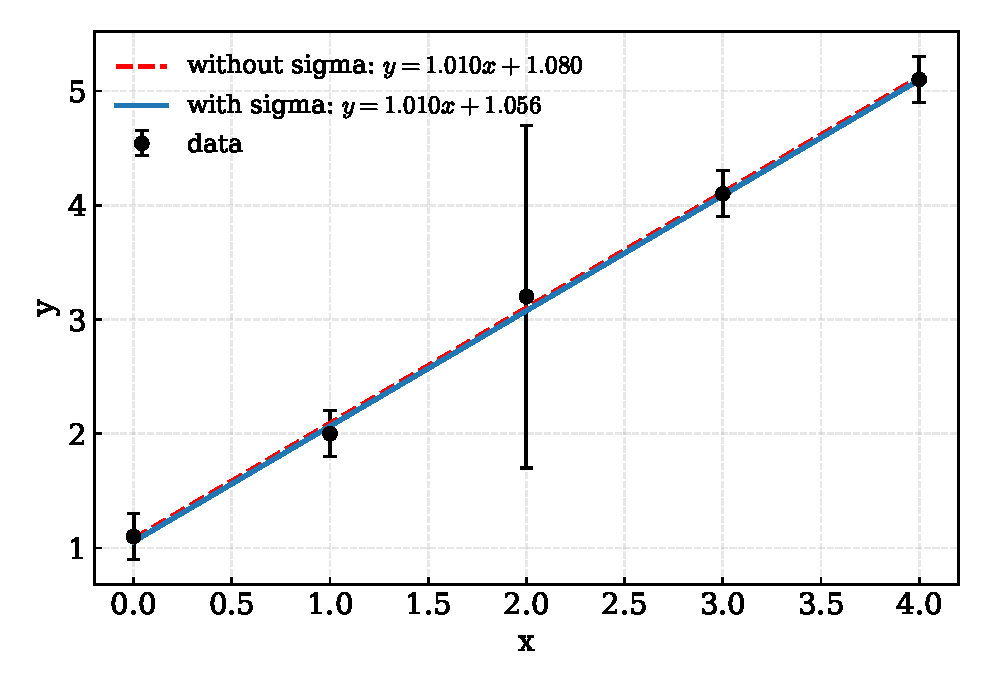
\includegraphics[width=0.7\linewidth]{fit_sigma_comparison.pdf}
\caption{\code{sigma} の有無によるフィット結果の違い。不確かさが点ごとに異なる場合、\code{sigma} の指定によって各残差の寄与が変わる。}
\label{fig:fit-sigma}
\end{figure}

\code{sigma} には、通常 \code{ydata} の各点に対応する 1 次元配列を渡す。このとき最小化される量は
\[
\chi^2(\mathbf{p}) = \sum_i
\left(
\frac{y_i - f(x_i; \mathbf{p})}{\sigma_i}
\right)^2
\]
と書けるので、\(\sigma_i\) が大きい点ほど目的関数への寄与は小さく、\(\sigma_i\) が小さい点ほど大きくなる。独立な Poisson 計数で平均値を観測数 \(N\) によって推定し、正規近似が妥当な範囲では、標準偏差を \(\sqrt{N}\) で近似する場合がある。低計数や重み付き計数には、その近似を機械的に適用しない。

\code{absolute\_sigma=True} は、共分散の計算に \code{sigma} の絶対的な大きさを使う指定である。渡した値が適切な標準偏差かどうかを、この設定が検証するわけではない。これを \code{False} のままにすると、\code{sigma} は相対的な重みとしては使われるが、共分散行列の大きさは残差のばらつきに合わせてあとから再スケーリングされる。そのため、推定値の重み付けだけでなく誤差評価まで行いたいなら、\code{sigma} の意味を明確にした上で \code{absolute\_sigma} の設定も意識する必要がある。

図~\ref{fig:fit-sigma} は、点ごとの不確かさを重みに反映した場合と、全点を等しい重みで扱った場合の違いを示している。どちらを採用するかは、\code{sigma} が測定の標準偏差を表すか、各点を同じ重みで比較する解析なのかによって決まる。

\code{curve\_fit()} の共分散とその対角成分から求める標準誤差は、解の近傍での線形近似に依存する~\cite{scipy_curvefit}。強い非線形性がある場合や、複数のパラメータを変えてもほぼ同じ曲線になる場合（パラメータ間の縮退）には、信頼できないことがある。1 次元の \code{sigma} による上の式は各点の誤差を独立とする。相関を扱うには共分散行列を渡す方法があり、通常の呼び出しは横軸 \code{xdata} の測定誤差を考慮しない。

\subsection{\code{scipy.interpolate} による補間}

補間は、測定点の間における値を仮定した関数形から推定する操作である。ここでは、1 次元データに対する区分線形補間を扱う。

\begin{lstlisting}[language=Python]
from scipy.interpolate import make_interp_spline

x = np.array([0.0, 1.0, 2.0, 4.0])
y = np.array([0.0, 2.0, 1.0, 3.0])

linear_interp = make_interp_spline(x, y, k=1)
x_new = np.array([0.5, 1.5, 3.0])
y_new = linear_interp(x_new, extrapolate=False)

print(y_new)
\end{lstlisting}

補間点 \code{x\_new} に対しては、次の値が返る。

\begin{lstlisting}[numbers=none, xleftmargin=2\zw]
[1.  1.5 2. ]
\end{lstlisting}

入力の \code{x} は重複がなく、昇順に並んでいる必要がある。区分線形補間は測定点を通る連続関数だが、接続点で傾きが不連続になり得る。上の \code{extrapolate=False} は入力範囲の外で \code{NaN} を返し、外挿を行わない指定である。範囲外まで同じ傾向が続くとは限らない。

線形補間では、各区間 \(x_i \le x \le x_{i+1}\) で
\[
y(x) = y_i + \frac{y_{i+1}-y_i}{x_{i+1}-x_i}(x-x_i)
\]
という一次式を使っている。したがって、測定点の間では直線でつながるが、測定範囲の外ではこの式をそのまま信じる根拠はない。

\subsection{\code{scipy.signal} による平滑化とピーク検出}

波形や時系列では、ピークの検出や軽い平滑化がよく必要になる。

\begin{lstlisting}[language=Python]
from scipy.signal import savgol_filter, find_peaks

x = np.linspace(0.0, 20.0, 200)
signal = np.sin(x) + 0.15 * np.random.default_rng(7).normal(size=x.size)

smooth = savgol_filter(signal, window_length=11, polyorder=3)
peaks, props = find_peaks(smooth, height=0.7, distance=15)

print(peaks)
print(np.round(props["peak_heights"], 3))
\end{lstlisting}

この例では、検出されたピーク位置とその高さが次のように表示される。

\begin{lstlisting}[numbers=none, xleftmargin=2\zw]
[ 13  76 138]
[0.977 1.048 0.994]
\end{lstlisting}

\code{savgol\_filter()} は局所多項式によって平滑化する。\code{find\_peaks()} は高さ、試料点間の距離、prominence などの条件でピーク候補を抽出する。検出条件をサンプリング間隔と対応付け、既知の合成波形で検出率と誤検出を確認してから実データへ適用する。

\subsection{\code{scipy.integrate} と \code{scipy.constants}}

\code{scipy.integrate} は離散点または関数の数値積分を、\code{scipy.constants} は物理定数の数値と単位情報を提供する。

\begin{lstlisting}[language=Python]
from scipy import constants
from scipy.integrate import simpson

x = np.linspace(0.0, np.pi, 101)
y = np.sin(x)

area = simpson(y, x=x)
print(area)
print(constants.c)
\end{lstlisting}

この積分値と光速定数は、次のように出力される。

\begin{lstlisting}[numbers=none, xleftmargin=2\zw]
2.0000000108245044
299792458.0
\end{lstlisting}

\code{simpson()} は、ここでは
\[
\int_0^\pi \sin x\,dx = 2
\]
という積分を、離散点 \((x_i, y_i)\) から数値的に評価している。したがって、\code{simpson(y, x=x)} は「\(y(x)\) をサンプル点から積分する関数」と読めばよい。また、\code{constants.c} は
\[
c = 299792458\ \mathrm{m\,s^{-1}}
\]
を表す定数である。\code{constants.c} 自体は単位を保持しない浮動小数点数なので、単位を演算中も保持する必要がある場合は、次章の Astropy の \code{Quantity} と定数オブジェクトを用いる。

\section{モデル・制約・外挿に関する注意点}

\subsection{モデル選択の理由がないままフィットしない}

ガウシアン、指数、直線の選択には、物理的または統計的な仮定が必要である。曲線がデータ点の近くを通ることだけでは、モデルの生成過程やパラメータの解釈を正当化できない。

\subsection{初期値と制約を無視しない}

非線形フィットは、初期値によって異なる極小値へ収束したり、収束しなかったりする。\code{curve\_fit()} が値を返したからといって、それが唯一の解だとは限らない。複数の初期値で試す、図へ重ねて見る、残差を見る、といった確認が必要である。

\subsection{補間と外挿を混同しない}

\code{make\_interp\_spline()} などの補間関数は、観測点の間を埋めるための道具である。測定範囲の外まで同じ関係が続く根拠は補間からは得られない。外側を予測する場合は、外挿に用いるモデルと適用範囲を別に検討する。

\subsection{信号処理におけるサンプリング間隔}

\code{find\_peaks()} の \code{distance} やフィルタ長は、サンプル数で指定することが多い。したがって、時間軸が 1 サンプル 1 ns なのか 10 ns なのかで、同じ数値でも意味が変わる。コード中の数字をそのまま流用せず、軸の単位へ戻して考える必要がある。

\section{発生間隔分布のモデル比較}

分布を比べる前に、解析に使う測定値の集まりを標本、その分布を決める調整値をパラメータ（母数）と呼ぶことを確認する。例えば、位置を 0 に固定した指数分布では、平均待ち時間が一つのパラメータになる。

図では、ある値以下に入る標本の割合を階段状に描くと、分布の形を比較できる。例えば 5 個の間隔のうち 3 個が 100 秒以下なら、100 秒での割合は \(3/5=0.6\) である。この図を経験累積分布関数（ECDF）と呼び、モデルの累積分布関数（CDF）と重ねる。次は、5 個の人工的な間隔を指数分布と比べる例である。

\begin{lstlisting}[language=Python]
import numpy as np
import matplotlib.pyplot as plt
from scipy import stats

intervals = np.array([30.0, 60.0, 90.0, 140.0, 360.0])
ordered = np.sort(intervals)
fraction = np.arange(1, len(ordered) + 1) / len(ordered)
loc, scale = stats.expon.fit(intervals, floc=0)
print(scale)

fig, ax = plt.subplots()
ax.step(ordered, fraction, where="post", label="data")
ax.plot(ordered, stats.expon.cdf(ordered, loc=loc, scale=scale),
        label="exponential model")
ax.set_xlabel("interval [s]")
ax.set_ylabel("cumulative fraction")
ax.legend()
fig.savefig("interval_cdf.pdf")
\end{lstlisting}

平均待ち時間の推定値は 136 秒となる。\code{fraction} は \code{[0.2, 0.4, 0.6, 0.8, 1.0]} であり、100 秒以下の割合は 0.6 である。\code{floc=0} は分布の開始位置を 0 秒へ固定する指定である。保存した図では、同じ横軸の値に対するデータとモデルの縦軸の差を比べる。少数の値で描画方法を確かめた後、実データでは標本数や独立性も考慮してモデルを判断する。

指数分布では、すでに \(c\) 秒待っても事象が起きていなければ、その後に待つ時間も元と同じ指数分布に従う。この性質を無記憶性という。したがって、\(t\geq c\) の間隔だけを使う場合は、起点を引いた \(t-c\) に対して平均待ち時間を推定する。

\subsection{補足：尤度と AIC による比較}

個々の値が互いに独立で同じ分布から得られたと仮定すると、各観測値での確率密度を掛け合わせ、パラメータによってデータとの合い方を比べられる。この積を尤度という。連続値では密度を使うので、尤度を「その値が出る確率」とは呼ばない。尤度を最大にするパラメータを探す方法が最尤推定であり、SciPy の連続分布の \code{fit()} は既定でこの方法を使う~\cite{scipy_distribution_fit}。計算では自然対数を取り、密度の積を \code{logpdf(...).sum()} という和へ変える。

調整するパラメータを増やすと、データへ合わせやすくなる。その複雑さも含めて候補を比べる指標の一つが AIC（赤池情報量規準）であり、\(\mathrm{AIC}=2k-2\log L\) と定義される~\cite{statsmodels_aic}。\(k\) はデータから推定したパラメータ数、\(L\) は最大尤度、\(\log\) は自然対数である。同じ標本と同じ観測範囲に対して求めた候補の間で、小さい値を選ぶ目安にする。AIC が小さいことだけでは、モデルの正しさは保証されない。地震間に相関があれば、上の独立性の仮定も別に検討する。

SciPy は、入力配列の物理的意味や、採用すべきモデルを自動では決めない。特にフィットでは、データ範囲、重み、残差、推定値の不確かさを確認し、採用した条件を結果とともに記録する必要がある。

本文を読み終えた後で関数名や引数を確認したいときは、SciPy User Guide~\cite{scipy_user_guide} を起点にすると探しやすい。分布や検定は Statistics~\cite{scipy_stats}、フィットや最適化は Optimization~\cite{scipy_optimize}、補間は Interpolation~\cite{scipy_interpolate}、波形処理は Signal processing~\cite{scipy_signal}、数値積分は Integration~\cite{scipy_integrate} が対応している。

\clearpage
\section{章末課題：モデルを当てはめて妥当性を確かめる}

本章の作業フォルダー \code{\textasciitilde/analysis\_practice/scipy} に、次を \code{scipy\_exercises.py} として保存する。各問の処理を追記し、\code{python scipy\_exercises.py} で実行する。1・2 問目にはこの人工データを使う。\code{synthetic\_dt} は秒単位の間隔、\code{y\_obs} は直線にばらつきを加えた測定値である。

\begin{lstlisting}[language=Python]
import numpy as np
from scipy import stats
from scipy.optimize import curve_fit

rng = np.random.default_rng(20260412)
synthetic_dt = rng.exponential(scale=120.0, size=5000)
x = np.linspace(0.0, 10.0, 80)
y_true = 2.5 * x + 1.2
sigma = np.full_like(x, 0.5)
y_obs = y_true + rng.normal(scale=sigma)
\end{lstlisting}

\begin{enumerate}
\item \begin{minipage}[t]{\linewidth}
\textbf{平均待ち時間を推定する。}
\code{stats.expon.fit(synthetic\_dt, floc=0)} の返り値から \code{scale} を取り出せ。生成時の平均 120 秒、\code{synthetic\_dt.mean()}、推定した \code{scale} を表にせよ。推定値が 115～125 秒に入ることを \code{assert} で確かめる。
\end{minipage}

\item \begin{minipage}[t]{\linewidth}
\textbf{直線を求め、残差を描く。}
\code{x} と \code{y\_obs} に \code{curve\_fit()} で直線を当てはめ、\code{sigma=sigma, absolute\_sigma=True} を指定せよ。上段に測定点と直線、下段に「測定値－直線の値」を描く。傾き・切片と標準不確かさを表にし、生成時の傾き 2.5、切片 1.2 と比較せよ。検算の目安は傾き 2.3～2.7、切片 0.7～1.7 である。
\end{minipage}

\item \begin{minipage}[t]{\linewidth}
\textbf{実データへ分布を当てはめる。}
第~\ref{chap:numpy}~章の発展課題で求めた地震の発生間隔を使う。ヒストグラムと経験累積分布を描き、指数分布と別の候補分布を当てはめて比較せよ。データがなければ \code{synthetic\_dt} を使う。経験累積分布とモデルの累積分布を重ね、同じ時刻での縦軸の差も描け。採用する分布と推定範囲を選んだ理由を述べよ。実カタログを使った場合は、期間、地域、件数、地震の種別、マグニチュード尺度を記す。
\end{minipage}

\item \begin{minipage}[t]{\linewidth}
\textbf{一つの解析条件を変えて比較する。}
3 問目のビン幅、推定範囲、重み、モデルのうち、自分の推定方法で使っている条件を一つ選んで変更せよ。変更した条件、推定値、不確かさを変更前後の表にする。範囲を限定する場合は、その範囲で規格化した条件付き分布を使う。指数分布で \(t\geq c\) だけを使う場合は、同モデルの無記憶性に基づき \(t-c\) へ当てはめる。
\end{minipage}

\item \begin{minipage}[t]{\linewidth}
\textbf{発展：地震規模と累積件数の関係を調べる。}
実カタログのマグニチュード \(M\) を使い、各値以上の地震数 \(N(\geq M)\) を数えて描け。小さい地震の取りこぼしが少ないと考える下限 \(M_c\) を選び、その上の範囲で \(\log_{10}N(\geq M)=a-bM\) の関係~\cite{gutenberg_richter_1944}を検討せよ。\(M_c\)、件数、推定法、不確かさ、図と残差を示す。累積件数の点は独立でないため、推定には個々の値の尤度か、重ならない区間の計数モデルを用いる。
\end{minipage}

\end{enumerate}
